\chapter{Akwizycja i wykorzystanie danych z czujników ruchu}

Celem tego rozdziału jest ukazanie, w jaki sposób zastosować odczyty prędkości kątowych, wartości przyspieszenia ziemskiego oraz natężenia ziemskiego pola magnetycznego, w poszczególnych osiach, tak aby uzyskać wartości kątów RPY, które wykorzystuje się do opisu rotacji względem układu XYZ. 

Przy niektórych obliczeniach, konieczne będzie dokonanie dodatkowych rotacji układu bazowego lub wektora względem, którego mierzymy rotację. W tym celu zastosowano macierze obrotów, których zapis dodatkowo uproszczono wprowadzając następujące oznaczenia
$$
    \begin{array}{ccc}
        s_{\varphi} = sin\varphi, & s_{\theta} = sin\theta, & s_{\psi} = sin\psi \\
        c_{\varphi} = cos\varphi, & c_{\theta} = cos\theta, & c_{\psi} = cos\psi
    \end{array}
$$

Macierze obrotów
$$
    \mathbf{R_x(\varphi)} =
    \left[
        \begin{array}{ccc}
            1 & 0 & 0 \\
            0 & c_{\varphi} & s_{\varphi} \\
            0 & -s_{\varphi} & c_{\varphi}
        \end{array}
    \right]
    \quad
    \mathbf{R_y(\theta)} =
    \left[
        \begin{array}{ccc}
            c_{\theta} & 0 & -s_{\theta} \\
            0 & 1 & 0 \\
            s_{\theta} & 0 & c_{\theta}
        \end{array}
    \right]
    \quad
    \mathbf{R_z(\psi)} =
    \left[
        \begin{array}{ccc}
            c_{\psi} & s_{\psi} & 0 \\
            -s_{\psi} & c_{\psi} & 0 \\
            0 & 0 & 1
        \end{array}
    \right]
$$

Złożenie macierzy obrotów wokół trzech osi jednocześnie
$$
    \mathbf{R} =
    \mathbf{R_x(\varphi)R_y(\theta)R_z(\psi)} =
    \left[
        \begin{array}{ccc}
            c_{\theta}c_{\psi} & c_{\theta}s_{\psi} & s_{\theta} \\
            c_{\psi}s_{\theta}s_{\varphi} - s_{\varphi}s_{\psi} & c_{\varphi}c_{\psi} + s_{\theta}s_{\varphi}s_{\psi} & c_{\theta}s_{\varphi} \\
            c_{\varphi}c_{\psi}s_{\theta} + s_{\varphi}s_{\psi} & c_{\varphi}s_{\theta}s_{\psi} - c_{\psi}s_{\varphi} & c_{\theta}c_{\varphi}
        \end{array}
    \right]
$$
%----------------------------------------------------------------------------------------------------------------
\section{Żyroskop}

Żyroskop prędkościowy mierzy prędkości kątowe w osiach własnego lokalnego układu współrzędnych, na podstawie, których możemy utworzyć wektor prędkości kątowych
$$
    \mathbf{\omega} = 
    \left[
    \begin{array}{c}
        \omega_x \\
        \omega_y \\
        \omega_z
    \end{array}
    \right]
$$
który dla prawidłowo skalibrowanego czujnika leżącego nieruchomo powinien być zerowy

Prędkości kątowe w poszczególnych osiach, jak i same osie układu współrzędnych żyroskopu, przedstawione zostały na rysunku \ref{Zyroskop oznaczenia}

\begin{figure}
    \centering
    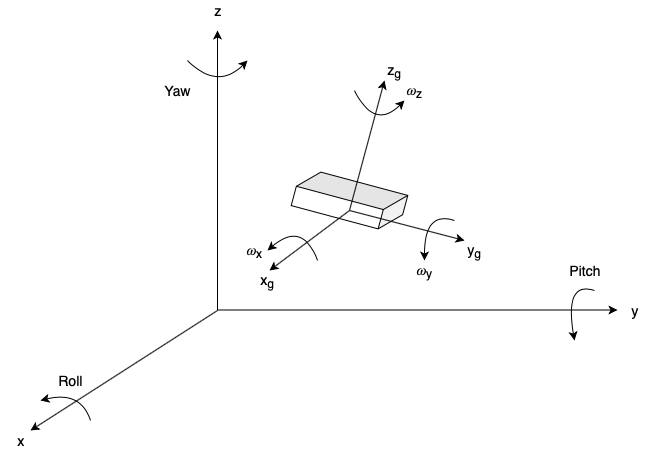
\includegraphics[width=0.6\textwidth]{Rysunki/Rozdzial03/Zyroskop.png}
    \caption{Wizualizacja odczytów żyroskopu}
    \label{Zyroskop oznaczenia}
\end{figure}

\newpage

W przypadku, w którym interesuje nas jednowymiarowe określenie rotacji, możemy je wyznaczyć poprzez scałkowanie prędkości kątowej w danej osi. W taki sposób otrzymamy wartość kąta obrotu wokół osi wyrażonej w radianach lub stopniach, w zależności od jednostki wyrażającej prędkość kątową \cite{Akwizycja}
$$
    \alpha_t = \int_{0}^{t} \omega \Delta t = \alpha_{t-1} + \omega_t \Delta t
$$

Problem pojawia się w momencie, w którym chcemy znać rotacje czujnika w przestrzeni trójwymiarowej. W momencie wprowadzenia rotacji czujnika względem układu bazowego i próbie wyliczenia rotacji wokół trzech osi układu bazowego, kąty obrotu wyznaczone na podstawie takich odczytów będą niepoprawne, ponieważ nie uwzględniają one rotacji lokalnego układu żyroskopu względem układu bazowego. W takim przypadku, należy zastosować wzór na prędkość kątową w przestrzeni \cite{Robotyka}
\begin{equation}
    \left[\omega\right] = \dot{R}R^T
    \label{Predkosc obrotowa}
\end{equation}
gdzie
$$
    \mathbf{\left[\omega\right]} = 
    \left[
    \begin{array}{ccc}
        0 & -\omega_z & \omega_y \\
        \omega_z & 0 & -\omega_x \\
        -\omega_y & \omega_x & 0
    \end{array}
    \right]
$$
Elementami równania (\ref{Predkosc obrotowa}), który chcemy wyznaczyć jest macierz rotacji. Dokonuje się tego poprzez przekształcenie go do postaci równania różniczkowego
$$
\dot{R} = R\left[\omega\right]
$$
korzystając z własności $R^T=R^{-1}$, wynikającej z ortogonalności macierzy \textbf{R}, którego przybliżonym rozwiązaniem jest
$$
    R_t \approx R_{t-1}(I_{3x3}+\left[\omega\right] \Delta t)
$$

$$
    \left[
    \begin{array}{ccc}
        r_{11} & r_{12} & r_{13} \\
        r_{21} & r_{22} & r_{23} \\
        r_{31} & r_{32} & r_{33} \\
    \end{array}
    \right]_t
    \approx
    \left[
    \begin{array}{ccc}
        r_{11} & r_{12} & r_{13} \\
        r_{21} & r_{22} & r_{23} \\
        r_{31} & r_{32} & r_{33} \\
    \end{array}
    \right]_{t-1}
    %
    \left[
    \begin{array}{ccc}
        1 & -\omega_z\Delta t & \omega_y\Delta t \\
        \omega_z\Delta t & 1 & -\omega_x\Delta t \\
        -\omega_y\Delta t & \omega_x\Delta t & 1 \\
    \end{array}
    \right]
$$
gdzie macierz $R_t$ w chwili $t=0$ (pierwsza iteracja) dla zerowych wartości kątów, wynosi
$$
    \mathbf{R_{0}} =
    \left[
    \begin{array}{ccc}
        1 & 0 & 0 \\
        0 & 1 & 0 \\
        0 & 0 & 1
    \end{array}
    \right]
$$

Mając przybliżone rozwiązanie równania różniczkowego, możemy obliczyć elementy macierzy $R_t$ oraz kąty Eulera na podstawie odpowiednich elementów tej macierzy
\begin{equation}
    \begin{array}{c}
        Roll(\varphi) = arctan(\frac{r_{32}}{r_{33}}) \\ \\
        Pitch(\theta) = arcsin(-r_{31}) \\ \\
        Yaw(\psi) = arctan(\frac{r_{21}}{r_{11}})
    \end{array}
\end{equation}

Z racji, tego że korzystamy z przybliżonego rozwiązania równania różniczkowego, wyznaczanego w sposób iteracyjny występuje problem normalizacji macierzy \textbf{R}. Problem ten został jednak pominięty ze względu na osiągnięta zadowalająca dokładność wyznaczanej rotacji na podstawie takiej, która nie zawsze jest znormalizowana.

%----------------------------------------------------------------------------------------------------------------
\section{Akcelerometr}

Akcelerometr mierzący przyspieszenie liniowe, wykorzystujemy do pomiaru przyspieszenia ziemskiego, które w przybliżeniu wynosi $1g$. Na podstawie odczytów z akcelerometru tworzymy wektor przyspieszeń w osiach jego lokalnego układu współrzędnych
$$
    \mathbf{a} = 
    \left[
    \begin{array}{cc}
        a_x \\
        a_y \\
        a_z
    \end{array}
    \right]
$$
Dla prawidłowo skalibrowanego czujnika leżącego nieruchomo, w którym wektor przyspieszenia ziemskiego jest równoległy do osi Z, wartość wektora w osi Z powinna wynosić 1, co oznacza przyspieszenie w tej osi równe 1g, a w osiach X oraz Y, wartość przyspieszenia powinna wynosić 0.

Do wyznaczenia rotacji czujnika względem układu bazowego służy wektor przyspieszenia ziemskiego, którego zwrot, kierunek i wartość są w przybliżeniu stałe. Dzięki temu w oparciu o zależności trygonometryczne między rozkładającym się tym wektorem na poszczególne osie w momencie wprowadzenia rotacji akcelerometru uzyskujemy wartości tych obrotów.

Rysunek poglądowy z oznaczeniami przyspieszeń, wektorów oraz osi, wprowadzonymi dla akcelerometru znajduje się na rysunku \ref{Akcelerometr oznaczenia}

\begin{figure}[!htb]
    \centering
    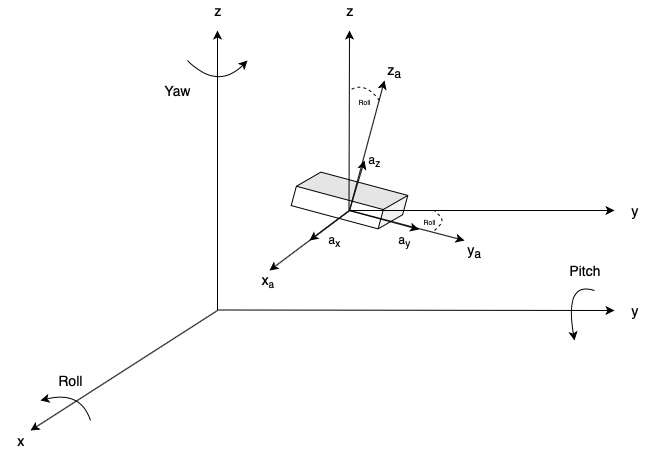
\includegraphics[width=0.6\textwidth]{Rysunki/Rozdzial03/Akcelerometr.png}
    \caption{Wizualizacja odczytów akcelerometru}
    \label{Akcelerometr oznaczenia}
\end{figure}

Znormalizowany wektor równoległy do osi Z, będący wektorem przyspieszenia ziemskiego
$$
    \mathbf{(g_z)} =
    \left[
        \begin{array}{c}
            0 \\
            0 \\
            1
        \end{array}
    \right]
$$

Orientacja w przestrzeni RPY znormalizowanego wektora grawitacji
$$
R g_z = 
\left[
    \begin{array}{ccc}
        c_{\theta}c_{\psi} & c_{\theta}s_{\psi} & s_{\theta} \\
        c_{\psi}s_{\theta}s_{\varphi} - s_{\varphi}s_{\psi} & c_{\varphi}c_{\psi} + s_{\theta}s_{\varphi}s_{\psi} & c_{\theta}s_{\varphi} \\
        c_{\varphi}c_{\psi}s_{\theta} + s_{\varphi}s_{\psi} & c_{\varphi}s_{\theta}s_{\psi} - c_{\psi}s_{\varphi} & c_{\theta}c_{\varpi}
    \end{array}
\right]
\left[
    \begin{array}{c}
        0 \\
        0 \\
        1
    \end{array}
\right]
= 
\left[
    \begin{array}{c}
        -s_{\theta} \\
        c_{\theta}s_{\varphi} \\
        c_{\theta}c_{\varphi}
    \end{array}
\right]
$$

Orientację akcelerometru mierzy się względem wektora grawitacji, dzięki czemu można zapisać, że
\begin{equation}
    \mathbf{a} =
    \left[
        \begin{array}{c}
            -s_{\theta} \\
            c_{\theta}s_{\varphi} \\
            c_{\theta}c_{\varphi}
        \end{array}
    \right]
    \Rightarrow
    n
    \left[
        \begin{array}{c}
            a_x \\
            a_y \\
            a_z
        \end{array}
    \right]
    =
    \left[
        \begin{array}{c}
            -s_{\theta} \\
            c_{\theta}s_{\varphi} \\
            c_{\theta}c_{\varphi}
        \end{array}
    \right]
    \label{Orientacja akcelerometru}
\end{equation}
gdzie

$a_x$ -- odczyt akcelerometru w osi x

$a_y$ -- odczyt akcelerometru w osi y

$a_z$ -- odczyt akcelerometru w osi z

$n = \frac{1}{\sqrt{a_x^2 + a_y^2 + a_z^2}}$ 


Korzystając ze wzoru (\ref{Orientacja akcelerometru}) zapisujemy go w postaci układu równań
$$
    \left\{
        \begin{array}{l}
            na_x = -sin\theta\\
            na_y = cos\theta sin\varphi\\
            na_z = cos\theta cos\varphi
        \end{array}
    \right.
    \Rightarrow
    \left\{
        \begin{array}{l}
            sin\theta = -na_x \\
            cos\theta = n\sqrt{a_y^2 + a_z^2} \\
            sin\varphi = \frac{na_y}{cos\theta} \\
            cos\varphi = \frac{na_z}{cos\theta}
        \end{array}
    \right.
$$
i wyliczamy zależności trygonometryczne, z których otrzymujemy rotację akcelerometru względem osi X oraz Y
\begin{equation}
    \begin{array}{l}
        tg\varphi = \frac{sin\varphi}{cos\varphi} = \frac{a_y}{a_z} \Rightarrow Roll(\varphi) = arctg(\frac{a_y}{a_z}) \\ \\
        tg\theta = \frac{sin\theta}{cos\theta} = \frac{-a_x}{\sqrt{a_y^2+a_z^2}} \Rightarrow Pitch(\theta) = arctg\left(\frac{-a_x}{\sqrt{a_y^2+a_z^2}}\right)
    \end{array}
\end{equation}

Z racji tego, że orientację akcelerometru wyliczamy względem wektora grawitacji, nie ma możliwości obliczenia rotacji względem osi Z, czyli kąta Yaw($\psi$).

%----------------------------------------------------------------------------------------------------------------
\section{Magnetometr}

Magnetometr jest urządzeniem mierzącym natężenie pola magnetycznego. Na podstawie odczytów z magnetometru możemy utworzyć wektor natężenia pola magnetycznego w poszczególnych osiach jego lokalnego układu współrzędnych
$$
    \mathbf{B} = 
    \left[
    \begin{array}{c}
        m_x \\
        m_y \\
        m_z
    \end{array}
    \right]
$$

Wprowadzone dla magnetometru oznaczenia, takie jak wartości natężeń pola magnetycznego w poszczególnych osiach, czy wektor północy magnetycznej przedstawione są na rysunku \ref{Magnetometr oznaczenia}

\begin{figure}[h!]
    \centering
    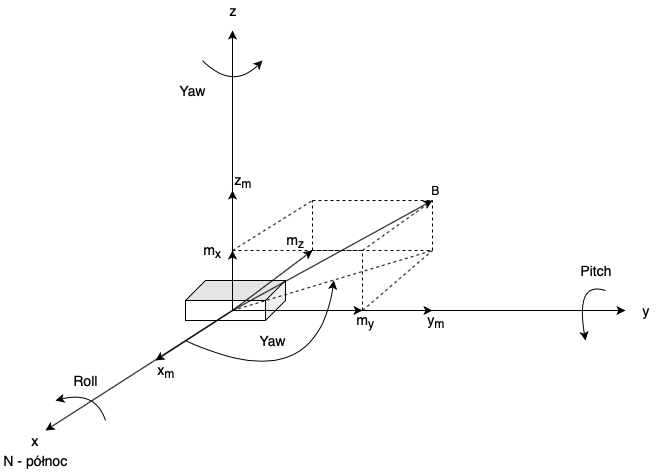
\includegraphics[width=0.6\textwidth]{Rysunki/Rozdzial03/Magnetometr.png}
    \caption{Wizualizacja odczytów magnetometru}
    \label{Magnetometr oznaczenia}
\end{figure}

Rotacja magnetometru wokół osi Z (odchylenie od wektora pola magnetycznego) przedstawionej na rysunku \ref{Rotacja magnetometru}, przy założeniu, że wartości kątów Roll i Pitch są zerowe (brak odchylenia magnetometru od płaszczyzny XY) wynosi
\begin{equation}
    tg\psi = \frac{sin\psi}{cos\psi} = \frac{m_y}{m_x} \Rightarrow Yaw(\delta) = arctg\left(\frac{m_y}{m_x}\right)
    \label{Odchylenie magnetometru}
\end{equation}

\begin{figure}[h!]
    \centering
    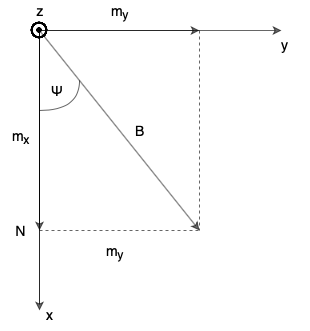
\includegraphics[width=0.3\textwidth]{Rysunki/Rozdzial03/Magnetometr_odchylenie.png}
    \caption{Odchylenie magnetometru od wektora północy magnetycznej}
    \label{Rotacja magnetometru}
\end{figure}

W przypadku, w którym odchylimy magnetometr względem osi X lub Y, obliczona według wzoru (\ref{Odchylenie magnetometru}) wartość obrotu wokół osi Z będzie nieprawidłowa, ponieważ zmieni się odczyt magnetometru w osiach X, Y oraz Z. W celu zniwelowania tego efektu dokonuje się kompensacji kąta wychylenia magnetometru.

%----------------------------------------------------------------------------------------------------------------
\subsection{Kompensacja kąta wychylenia}
Kompensacja kąta wychylenia magnetometru, to nic innego jak uwzględnienie w obliczeniach rotacji wokół osi X i Y, wyznaczonych, np. za pomocą akcelerometru.

Wektor pola magnetycznego po kompensacji kąta wychylenia ma postać
\begin{equation}
    \begin{array}{c}
        \mathbf{B^{k}} = R_x(\varphi)R_y(\theta)B 
        \\ \\
        \left[
            \begin{array}{c}
                b^k_x \\
                b^k_y \\
                b^k_z
            \end{array}
        \right]
        =
        \left[
            \begin{array}{ccc}
                c_{\theta} & 0 & -s_{\theta} \\
                s_{\varphi}s_{\theta} & c_{\varphi} & s_{\varphi}c_{\theta} \\
                c_{\varphi}s_{\theta} & -s_{\varphi} & c_{\varphi}c_{\theta}
            \end{array}
        \right]
        \left[
            \begin{array}{c}
                m_x \\
                m_y \\
                m_z
            \end{array}
        \right]
        =
        \left[
            \begin{array}{c}
                c_{\theta}m_x - s_{\theta}m_z \\
                s_{\varphi}s_{\theta}m_x + c_{\varphi}m_y + s_{\varphi}c_{\theta}m_z \\
                c_{\varphi}s_{\theta}m_x - s_{\varphi}m_y + c_{\varphi}c_{\theta}m_z
            \end{array}
        \right]
    \end{array}
\end{equation}

Rotacja magnetometru wokół osi Z (odchylenie od wektora pola magnetycznego), po kompensacji kąta wychylenia magnetometru
\begin{equation}
    Yaw(\psi) = arctg\left(\frac{b^k_y}{b^k_x}\right) = arctg\left(\frac{s_{\varphi}s_{\theta}m_x + c_{\varphi}m_y + s_{\varphi}c_{\theta}m_z}{c_{\theta}m_x - s_{\theta}m_z}\right)
    \label{Odchylenie po kompensacji}
\end{equation}

%----------------------------------------------------------------------------------------------------------------
\subsection{Deklinacja magnetyczna}
W celu uzyskania dokładniejszego pomiaru uzależnionego od aktualnej pozycji na Ziemi uwzględnia się deklinację magnetyczną, która obecnie dla Wrocławia wynosi (źródło Port Lotniczy Wrocław S.A.)
$$
    \delta = 4^{o}E8'E \approx 4,13^{o}E
$$
co daje ostateczną postać wzoru na wskazanie magnetometru, przy założeniu, że kąt Yaw obliczony jest w stopniach, a nie w radianach
$$
   Yaw(\psi) = Yaw(\psi) + \delta = Yaw(\psi) + 4,13^o 
$$

%----------------------------------------------------------------------------------------------------------------
\subsection{Kompensacja efektu ,,Hard Iron'' oraz ,,Soft Iron''}

Nieskalibrowane odczyty magnetometru zostały przedstawione na rysunku \ref{Magnetometr nieskalibrowany}. Na wykresach widoczne są elipsy przesunięte względem punktu (0,0) na wykresie, oraz delikatne zniekształcenia. Odczyty dla skalibrowanego magnetometru na płaszczyznach XY, XZ oraz YZ powinny mieć swój środek w punkcie (0,0), oraz nie powinny występować zniekształcenia. Odczyty w przestrzeni XYZ powinny być kulą o środku w punkcie (0,0,0).

Efekt ,,Hard Iron'' -- wpływ ferromagnetyków twardych, wytwarzających stałe pole magnetyczne. Objawia się on przesunięciem odczytów względem środka układu współrzędnych. Kompensuje się go poprzez przesunięcie odczytów na środek układu współrzędnych o wyznaczony offset. Przesunięcie wyznacza się na podstawie maksymalnej oraz minimalnej wartości odczytu w danej osi, według następujących wzorów
$$
    \begin{array}{c}
        \delta_x = \frac{max(m_x) + min(m_x)}{2} \\ \\
        \delta_y = \frac{max(m_y) + min(m_y)}{2} \\ \\
        \delta_z = \frac{max(m_z) + min(m_z)}{2}
    \end{array}
$$

Efekt ,,Soft Iron'' -- wpływ ferromagnetyków miękkich, który objawia się zniekształceniem odczytów, które powinny tworzyć idealny okrąg na płaszczyźnie. Kompensuje się go poprzez przeskalowanie odczytów o wartości wyliczane według następujących wzorów
$$
    \begin{array}{c}
        a_x = \frac{max(m_x) - min(m_x)}{2}
        \quad
        a_y = \frac{max(m_y) - min(m_y)}{2}
        \quad
        a_z = \frac{max(m_z) - min(m_z)}{2} \\ \\
        b = \frac{a(m_x) + a(m_y) + a(m_z)}{3} \\ \\
        s_x = \frac{b}{a(m_x)}
        \quad
        s_y = \frac{b}{a(m_y)}
        \quad
        s_z = \frac{b}{a(m_z)} 
    \end{array}
$$

Na rysunku \ref{Magnetometr skalibrowany} widać, że odczyty dla magnetometru zostały skalibrowane. Przesunięcia odczytów we wszystkich osiach oraz delikatne zniekształcenie dla odczytu XZ zostały skompensowane. Ostateczną postać wektora odczytów magnetometru oblicza się według wzoru
$$
    \begin{array}{c}
        \left[
            \begin{array}{c}
                m_x \\
                m_y \\
                m_z
            \end{array}
        \right]
        =
        \left[
            \begin{array}{c}
                m_x - \delta_x \\
                m_y - \delta_y \\
                m_z - \delta_z
            \end{array}
        \right]
        \left[
            \begin{array}{c}
                s_x \\
                s_y \\
                s_z
            \end{array}
        \right]
    \end{array}
    \label{Ostateczny wektor magnetometr}
$$

\begin{figure}[h!]
    \centering
    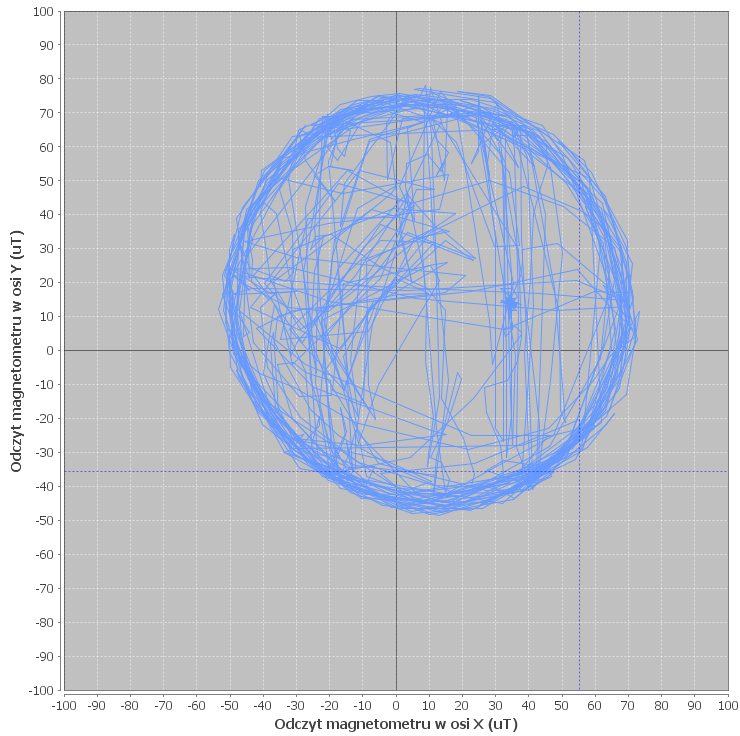
\includegraphics[width=0.5\textwidth]{Rysunki/Rozdzial03/Magnetometr_nieskalibrowany_XY.png}
    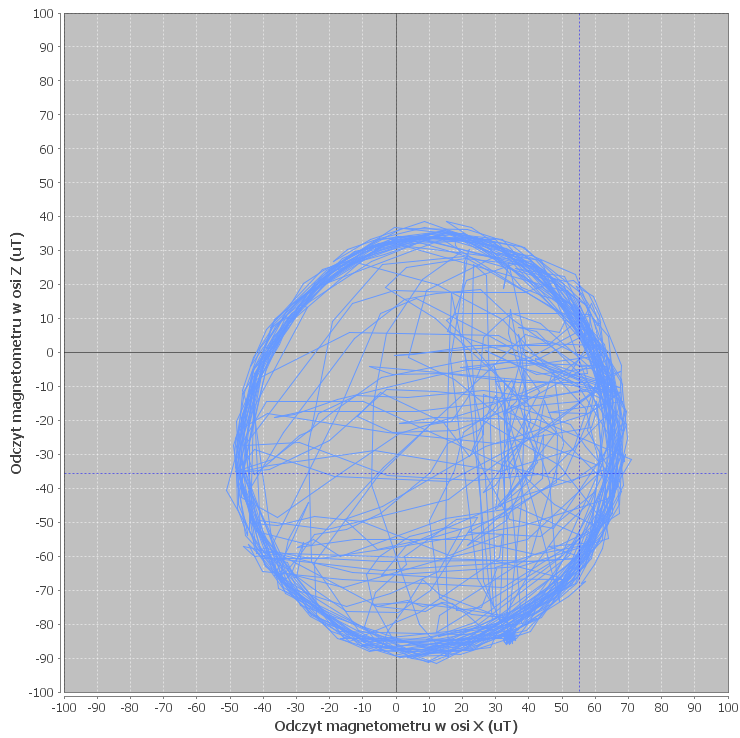
\includegraphics[width=0.5\textwidth]{Rysunki/Rozdzial03/Magnetometr_nieskalibrowany_XZ.png}
    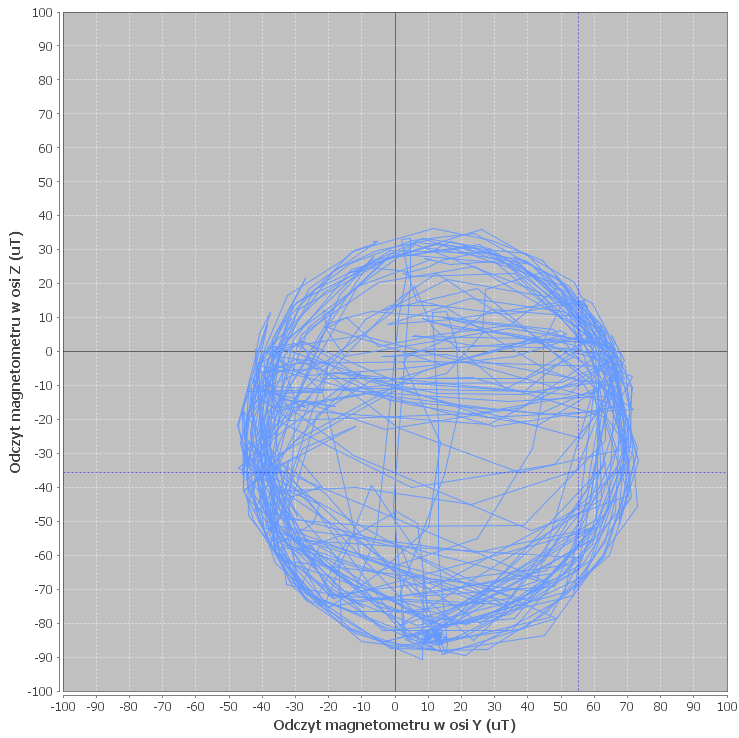
\includegraphics[width=0.5\textwidth]{Rysunki/Rozdzial03/Magnetometr_nieskalibrowany_YZ.png}
    \caption{Odczyty dla nieskalibrowanego magnetometru}
    \label{Magnetometr nieskalibrowany}
\end{figure}

\begin{figure}[h!]
    \centering
    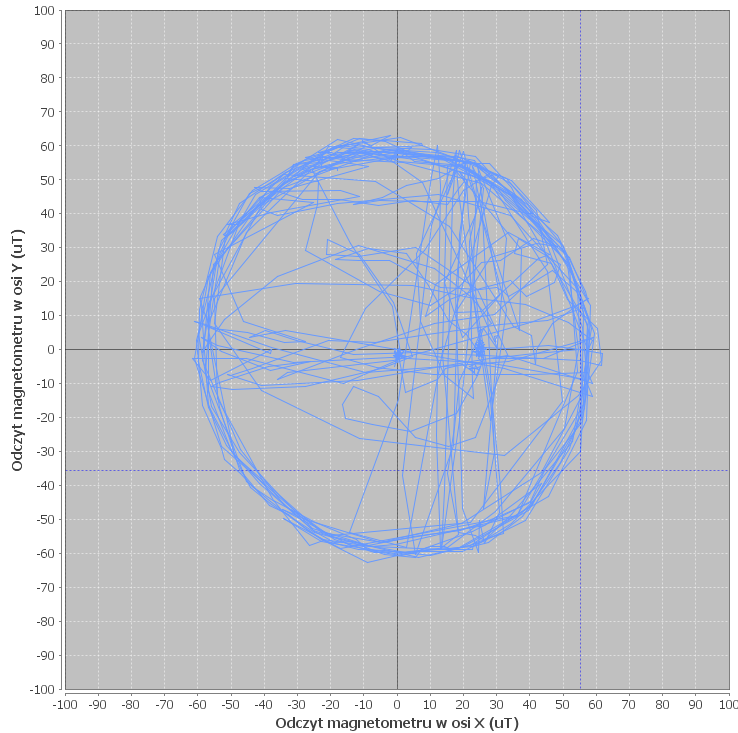
\includegraphics[width=0.5\textwidth]{Rysunki/Rozdzial03/Magnetometr_skalibrowany_hardiron_XY.png}
    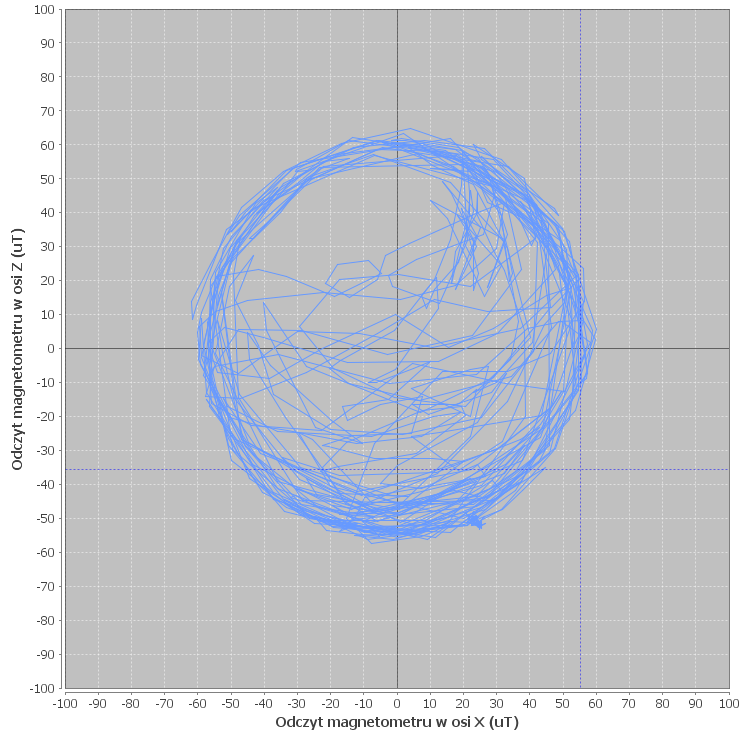
\includegraphics[width=0.5\textwidth]{Rysunki/Rozdzial03/Magnetometr_skalibrowany_hardiron_XZ.png}
    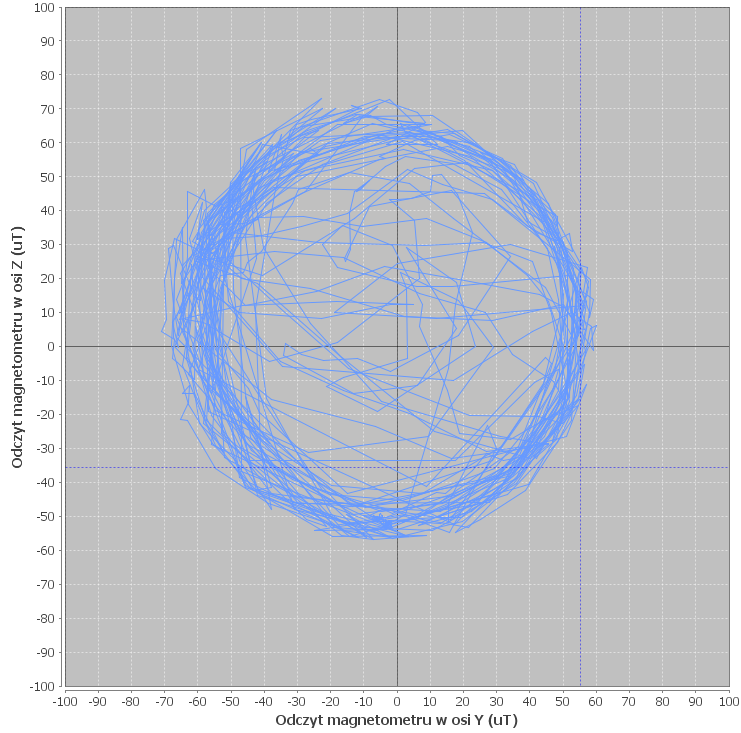
\includegraphics[width=0.5\textwidth]{Rysunki/Rozdzial03/Magnetometr_skalibrowany_hardiron_YZ.png}
    \caption{Odczyty dla skalibrowanego magnetometru}
    \label{Magnetometr skalibrowany}
\end{figure}

%----------------------------------------------------------------------------------------------------------------